\section{Saturation-induced finite-amplitude instability}\label{sec:bistability}

A step entry, by saturating the command, tips cuts that the linear analysis calls stable into chatter (Section~\ref{sec:feasibility}). This section measures how large a disturbance the settled cut tolerates under the DVF law of Eq.~\eqref{eq:dvf} with its hard clip, what happens beyond it, and how the tolerated disturbance depends on the residual authority. A cut is said to show \emph{finite-amplitude instability} when its forced orbit is linearly stable but a finite perturbation ends in chatter, and to be \emph{bistable} when, in addition, that chatter is a bounded attractor (Section~\ref{sec:bistab-attr}).

\subsection{Simulation protocols}\label{sec:bistab-prot}

All runs use the simulator of \ref{app:simulator}, the gains of Section~\ref{sec:feasibility} ($\mathcal G=[0,1500]$) and, unless stated otherwise, the clipped command. In the \emph{step entry} the full depth and immersion act from $t=0$, starting from rest with zero history. In the \emph{face entry} the tool advances into a workpiece face normal to the feed and reaches full engagement after 40 revolutions. In the \emph{feed ramp} the feed per tooth rises linearly from zero to $f_z$ over ten revolutions. The depth limit of an entry was found on a ladder of depths up to $1.05\alim$, refined by bisection (Supplementary Material), each run being judged over the 300 revolutions after the entry.
% src: src/tdsim.c (opt[1]-opt[3]: ramp_f, f0, edge), src/tdsim.py (entry_revs), src/c1_unsafe_zone.py (ENTRIES, LADDER), src/tdboundary.py (boundary, classify: rtol 3e-3, NREV 300); README §11.2

In the kick protocol the cut was settled by a face entry, and at revolution 100 a velocity increment $\Delta v$, the \emph{kick}, was added to $\dot x$ at one of 16 phases $\theta$ per tooth period; the 300 revolutions after it were classified. The \emph{critical kick} $\Delta v^*(\theta)$ is the smallest kick that ends in chatter; as the outcome is not monotone in $\Delta v$ (a large kick throws the tool out of the cut), it was found by an upward search up to \SI{3}{\metre\per\second} (Supplementary Material). The lower edge of the \emph{unsafe band}, in the sense of the unsafe zones of milling \citep{dombovari2015bistable,dombovari2019experimental}, was mapped every \SI{20}{\rpm} (126 speeds) as the smallest depth at which one of seven kicks from \SI{3}{\milli\metre\per\second} to \SI{3}{\metre\per\second} ends in chatter. The checks of these protocols asked for in the literature on bistable zones (kick timing, number of phases, window length, holes in the band) are collected in Section~\ref{sec:bistab-checks}.
% src: src/c1_unsafe_zone.py (KICK_REV = 100, WINDOW = 300, N_PHASE = 16, DV_GRID, N_BISECT = 6, BAND_STEP = 20, BAND_DV, BAND_PHASES = 2, BAND_BISECT = 6, _critical_kick, _band_low)

As a kick or an entry transient can throw the tool out of the cut for many passes, the chip is cut against the deepest earlier pass at the same angle [Eq.~\eqref{eq:surf}] \citep{tlusty1981basic}, a full memory without which clipped chatter can grow spuriously beyond \SI{1}{\centi\metre} (\ref{app:simulator}; Supplementary Material); only the off-axis runs of Section~\ref{sec:cert-c3} used the last four passes (\ref{app:lmi}). A run whose displacement exceeds \SI{1}{\centi\metre}, 200 feeds, is stopped and counted as chatter: such an excursion is a failure of the cut, whatever the model, far outside its validity, would do afterwards. Runs are classified by the criterion D1 of \ref{app:simulator}, which biases step-entry boundaries near $\alim$ high, by \SIrange{0.05}{1.5}{\percent} and by up to \SI{4.4}{\percent} near the forced resonance, but not kick-based limits or clipped limits well below $\alim$.
% src: README §11.2; verification/tdsim/check9_full_memory.json (bounded clipped chatter 0.43-0.59 mm with full memory and brute force; 1050 rpm, 0.9 a_lim diverges with both; nreg 4: 2 of 4 diverge, 0.554 vs 0.435 mm); src/tdboundary.py; verification/tdsim/check8_onset_long_runs.json (bias 0.05-1.47 %), check10_forced_resonance_long_runs.json (up to 4.4 %)

\subsection{The same cut, two outcomes}\label{sec:bistab-two}

At \SI{2500}{\rpm} with $g=1500$ ($\alim=\SI{17.24}{\milli\metre}$) and $a=\SI{15}{\milli\metre}$, the step entry ends in clipped chatter of about \SI{0.43}{\milli\metre}, whereas the face entry settles on the forced orbit with a command of about \SI{5}{\volt}. Figure~\ref{fig:two} shows the settled cut at $0.9\alim$, kicked just below and just above the critical kick of that phase, \SI{7.29}{\milli\metre\per\second}: after the smaller kick the motion returns to the forced orbit although the command still reaches the clip, after the larger one it grows into clipped chatter. The forced orbit and clipped chatter therefore coexist, and in this linear-force model, at kicks of this size, it is the saturation that makes them coexist: without the clip, chatter required kicks at least 50 times larger (Section~\ref{sec:bistab-basin}). The mechanism is a loss of effective gain (Section~\ref{sec:bistab-df}): once the chatter component, added to $b(t)$, reaches $\Vmax$, the clip passes on only part of the feedback, and the growing chatter saturates the command further.
% src: README §11.3; verification/tdsim/check9_full_memory.json (2500 rpm, 15 mm, step entry, full memory: max |x| = 0.435 mm); paper/figures/figure_numbers.json (fig03: 0.9 a_lim = 15.51 mm, kicks 7.0/7.6 mm/s at phase 0, critical kick 7.29 mm/s); results/c1_basin.npz (2500 rpm, 0.9 a_lim, clipped: phase 0 7.288 mm/s); closed form of Eq. (xp) gives b_max = 5.37 V at 15 mm (cross-check of README "about 5 V"); ratio 50: results/c1_basin.npz (smallest ratio of unclipped to clipped minimum kick, 52.1)

\begin{figure}[!tbp]
  \centering
  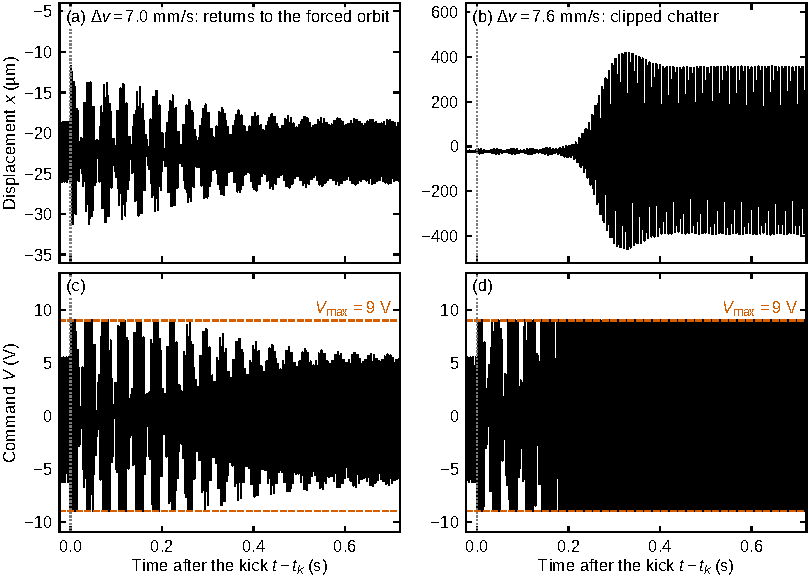
\includegraphics[width=\textwidth]{figures/fig03_two_outcomes.pdf}
  \caption{The same linearly stable cut (\SI{2500}{\rpm}, $g=\SI{1500}{\volt\second\per\metre}$, $a=0.9a_{\lim}=\SI{15.51}{\milli\metre}$, $\lvert V\rvert\le\SI{9}{\volt}$), settled by a face entry and kicked at the start of a tooth period, where the critical kick is \SI{7.29}{\milli\metre\per\second}. (a,\,c)~$\Delta v=\SI{7.0}{\milli\metre\per\second}$: the motion returns to the forced orbit. (b,\,d)~$\Delta v=\SI{7.6}{\milli\metre\per\second}$: it ends in clipped chatter. Top: displacement $x$; bottom: applied command $V$ and the clip $\pm V_{\max}$; dotted vertical line: the kick.}
  \label{fig:two}
\end{figure}
% src: paper/figures/figure_numbers.json (fig03), results/c1_basin.npz

\subsection{Entry limits over 251 speeds}\label{sec:bistab-map}

With the step entry the ratio of the clipped limit to $\alim$ has a median of 0.910 and a minimum of 0.736 (\SI{2460}{\rpm}), and it is below $0.97\alim$ at 157 of 251 speeds (Fig.~\ref{fig:map}). The face entry reaches at least $0.985\alim$ at every speed, and the feed ramp falls below $0.97\alim$ only at \SI{2000}{\rpm} ($0.957\alim$). Where the step entry binds, the better of the face entry and the feed ramp gains \SI{2.5}{\milli\metre} on average and up to \SI{4.7}{\milli\metre} (\SI{1980}{\rpm}). Without the clip the step-entry limit sits at the linear limit (median ratio 1.01; Supplementary Material).
% src: results/c1_map.npz, results/c1_summary.json (map: step_clip, edge_clip, feed_clip, step_free, soft_minus_step_mean_mm 2.51); results/c1_map.npz recomputed: largest gain of max(face, feed ramp) over the step entry where it binds 4.741 mm at 1980 rpm (19.02 vs 23.75 mm; 4.24 mm at 2500 rpm, 13.00 vs 17.25 mm); results/c1_map.npz recomputed: a_step_free/a_lim > 1.015 at 75 speeds (1.0165-1.050); a_edge_clip and a_feed_clip = 1.05 a_lim at 500, 540, 670, 720, 1000, 1080 rpm, a_step_clip at 500, 550, 670, 1000 rpm (seven speeds in all); at the other 245 speeds a_edge_clip mean 18.200 mm, a_lim mean 18.206 mm; results/feas_g1500.npz (at_bound: 157) vs results/c1_map.npz (a_step_clip < 0.97 a_lim: 157), 110 in common; verification/tdsim/check10_forced_resonance_long_runs.json

The lower edge of the unsafe band was found at 109 of the 126 speeds, at 0.21--$0.98\alim$ (median 0.46), and always above the uncontrolled limit, at no less than $1.08\alim(0)$. That the clip cannot create chatter below $\alim(0)$ is suggested by a describing-function argument, as the clip can only lower the effective gain, and is proved for the averaged model below a depth close to $\alim(0)$ in Section~\ref{sec:cert-global}. Above $\alim(0)$ a bounded basin is expected, since the uncontrolled cut is exponentially unstable there and no bounded input can stabilise it globally \citep{hu2001book}; what the simulations add is the size of the basin and its dependence on depth, speed and entry. No band was found at 17 speeds, most of them where the gain is small (Supplementary Material). The edge rests on kicks of up to \SI{3}{\metre\per\second}, far beyond the validity of the model; a scan of the depth confirms that the band has no holes (Section~\ref{sec:bistab-checks}). The step entry exposes only the top of the band, where the entry transient exceeds the basin.
% src: results/c1_band.npz, results/c1_summary.json (band: found 109/126, ratio 0.21/0.46/0.98, over_alim0_min 1.08, none_at_rpm, g_where_none); README §11.4

\begin{figure}[!tbp]
  \centering
  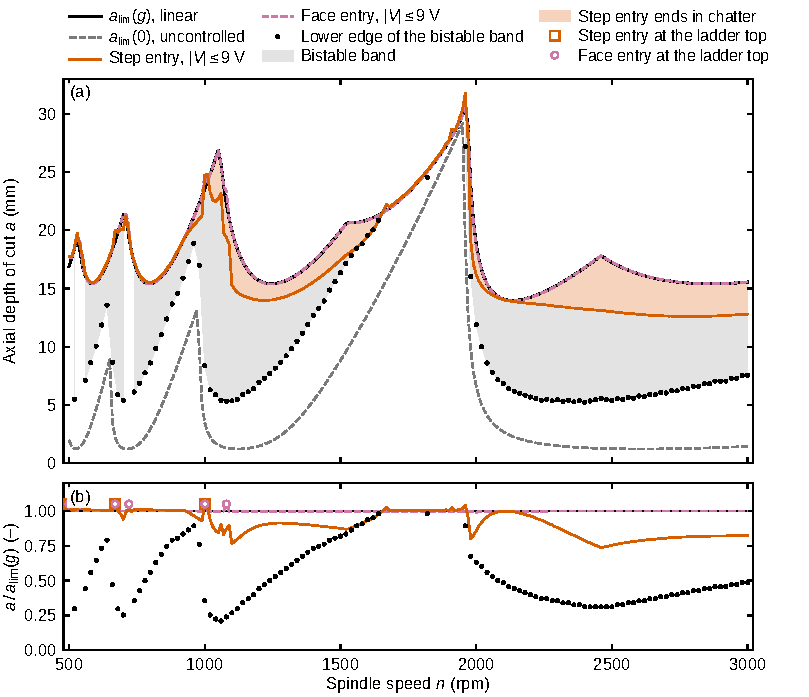
\includegraphics[width=\textwidth]{figures/fig04_entry_map.pdf}
  \caption{Depth limits over 251 speeds with the gains of Section~\ref{sec:feasibility} ($\mathcal G=[0,1500]$). (a)~Linear limit $a_{\lim}(g)$ and uncontrolled limit $a_{\lim}(0)$; time-domain limits with the \SI{9}{\volt} clip for the step entry and the face entry; lower edge of the unsafe band from kicks of \SI{3}{\milli\metre\per\second} to \SI{3}{\metre\per\second} on the settled cut (every \SI{20}{\rpm}). Shaded: the unsafe band, and the part of it in which the step entry ends in chatter. (b)~The same limits as fractions of $a_{\lim}(g)$; open markers: step-entry (squares) and face-entry (circles) limits at the top of the depth ladder, $1.05a_{\lim}$, above which they were not resolved.}
  \label{fig:map}
\end{figure}

\subsection{Basin of the forced orbit}\label{sec:bistab-basin}

Figure~\ref{fig:basin} and Table~\ref{tab:basin} give the critical kick at 1090, 1420, 2500 and \SI{2870}{\rpm} with $g=1500$, at twelve depths from 0.15 to $0.98\alim$ with the clip and at four without it. With the clip the basin is finite from 0.25--$0.80\alim$ onwards and narrows towards the limit. To give the kick a physical scale, its impulse $m\Delta v^*$ is compared with the mean cutting impulse of one tooth period,
\begin{equation}\label{eq:impulse}
  \bar F_yT,\qquad \bar F_y=\frac{N_t\,a\,f_z}{2\pi}\Bigl(\frac{\pi}{4}K_{tc}+\frac12K_{rc}\Bigr),
\end{equation}
where $\bar F_y$ is the mean static force normal to the feed. At $0.98\alim$ the critical kick of the worst phase carries \SIrange{2.4}{10.8}{\percent} of this impulse; as an equivalent displacement $\Delta v^*/\omega_n$ it is 2.9--\SI{13}{\micro\metre}, against a forced vibration of about \SI{4}{\micro\metre} amplitude at \SI{2500}{\rpm} and $0.9\alim$ (Fig.~\ref{fig:two}) and a feed of \SI{50}{\micro\metre}. Kicks of at most \SI{10}{\milli\metre\per\second} (\SI{12}{\micro\metre}) end in chatter only from 0.90--$0.95\alim$ upwards, if at all (Supplementary Material). Over the 16 phases the critical kick varies by at most \SI{24}{\percent}, so the basin is a property of the cut rather than of the timing of the disturbance.
% src: results/c1_basin.npz (dv, frac, vmax, tooth_impulse, mass), results/c1_summary.json (basin: first_finite_frac, impulse_098_pct, impulse_098_min_pct, phase_spread_098, phase_spread_max); src/c1_unsafe_zone.py (run_basin: tooth impulse); verification/paper/revision_runs.json (stored.kick_displacement_098: worst-phase dv at 0.98 a_lim 10.88, 5.04, 2.34, 8.12 mm/s = 13.4, 6.2, 2.9, 10.0 um at omega_n = 2 pi 129.3 rad/s, 1090/1420/2500/2870 rpm; recomputed from results/c1_basin.npz); results/c1_basin.npz recomputed: smallest depth with worst-phase dv <= 10 mm/s: 0.95, 0.90, 0.95 a_lim at 1420, 2500, 2870 rpm, none at 1090; <= 30 mm/s: 0.40, 0.80, 0.40, 0.50 a_lim at 1090, 1420, 2500, 2870 rpm; 10 mm/s / omega_n = 12.3 um; paper/figures/figure_numbers.json (fig03 orbit_x_um -26.0 to -18.6, i.e. 3.7 um amplitude)

\begin{table}[!tbp]
  \centering
  \caption{Critical kick $\Delta v^*$ of the clipped cut ($g=\SI{1500}{\volt\second\per\metre}$, $\lvert V\rvert\le\SI{9}{\volt}$): median over 16 phases and, in parentheses, the worst phase. The last column gives $m\Delta v^*$ as a percentage of the cutting impulse $\bar F_yT$ of Eq.~\eqref{eq:impulse}. Basin finite from: the smallest of the 12 depths at which some kick of at most \SI{3}{\metre\per\second} ends in chatter.}
  \label{tab:basin}
  \begin{tabular}{@{}rcccc@{}}
    \toprule
    Speed & Basin finite & \multicolumn{2}{c}{$\Delta v^*$ (\si{\milli\metre\per\second})} & $m\Delta v^*/(\bar F_yT)$ (\si{\percent})\\
    \cmidrule(lr){3-4}
    (rpm) & from $a/a_{\lim}$ & $a=0.9a_{\lim}$ & $a=0.98a_{\lim}$ & $a=0.98a_{\lim}$\\
    \midrule
    1090 & 0.25 & 15.3 (15.1) & 11.5 (10.9) & 4.3 (4.0)\\
    1420 & 0.80 & 13.7 (12.5) & 5.3 (5.0)   & 3.0 (2.9)\\
    2500 & 0.40 & 8.3 (7.2)   & 2.5 (2.3)   & 2.6 (2.4)\\
    2870 & 0.50 & 11.8 (11.5) & 8.7 (8.1)   & 11.5 (10.8)\\
    \bottomrule
  \end{tabular}
\end{table}
% src: results/c1_basin.npz; results/c1_summary.json (basin); README §11.5

Without the clip, no kick up to \SI{3}{\metre\per\second} ended in chatter at 13 of the 16 tested points; at the other three only kicks of 0.78--\SI{3}{\metre\per\second} in one phase did, the loss-of-contact bistability of milling without an actuator \citep{dombovari2015bistable}. In this linear-force model the clip thus shrinks the basin by a factor of 52--701 where the unclipped cut is itself bistable, and creates the bistability, on this range of kicks, at nine further points (Supplementary Material).
% src: results/c1_basin.npz (vmax = 0 rows; ratios of the smallest unclipped to the smallest clipped kick: 52.1, 275.7, 700.9; lower bounds 3 m/s / clipped minimum: 69.7-594.9); README §11.5

\subsection{What lies beyond the basin}\label{sec:bistab-attr}

The classifier shows that the basin is bounded, not where a trajectory that leaves it goes. At the 29 points of Table~\ref{tab:basin} where the basin is finite, the settled cut was therefore kicked at the worst phase with 2, 2.5 and 3 times the critical kick and followed for 2000 revolutions with the full surface memory. All 87 runs ended in bounded chatter whose statistics in the second and in the last quarter of the run agree (root mean square of $x$ and of $V$ within \SI{10}{\percent}, clipped fraction of the time within 0.05, chatter frequency within \SI{1}{\hertz}); none exceeded \SI{1}{\centi\metre} and none returned to the forced orbit. The chatter does not depend on the kick, its root mean square displacement differing by less than \SI{0.09}{\percent} between the three kicks. It keeps the command on the clip for 89--\SI{99}{\percent} of the time, at 133--\SI{153}{\hertz}, with a peak-to-peak displacement of 0.08--\SI{2.0}{\milli\metre}, far larger than the feed per tooth, so that the tool leaves the cut periodically, which bounds the amplitude \citep{tlusty1981basic}; at least \SI{98}{\percent} of its energy is not synchronous with the tooth passing. Continued to 4000 revolutions at the four points at $0.9\alim$, its root mean square and frequency change by less than \SI{0.13}{\percent} and \SI{0.003}{\hertz}. At these points the clipped cut is therefore bistable in the strict sense: the forced orbit coexists with a bounded, stationary chatter attractor (Fig.~\ref{fig:attr}).
% src: verification/paper/attractors_kick.json (summary: 29 points run, 87 runs, outcome_counts bounded_stationary 87; Q4 pp_x 0.081-1.993 mm, rms_V 8.67-8.98 V, clip_frac 0.891-0.992, f_chatter 132.7-153.1 Hz, nonsync_frac >= 0.978; max_rel_spread_rms_x_over_kicks <= 8.9e-4; long_runs at 0.9 a_lim: rel_change_rms_x <= 1.3e-3, change_f_chatter <= 2.0e-3 Hz)

Bifurcation-type diagrams against the depth place these attractors over the whole range (Fig.~\ref{fig:attr}a--d). At 28 depths from $\alim(0)$ to $1.05\,\alim$, the cut was started by a face entry, by the same with a kick of 0.03 or \SI{0.3}{\metre\per\second} at revolution 100, and by a step entry, and was run for 1600 revolutions. Every start ended either on the forced orbit or in bounded, stationary chatter; none exceeded \SI{1}{\centi\metre}. The chatter branch, reached from at least one start, begins at 0.25, 0.74, 0.31 and $0.44\,\alim$ at 1090, 1420, 2500 and \SI{2870}{\rpm} (its lower ends refined by bisection, consistent with the coarser depth grid of Table~\ref{tab:basin}) and coexists with the forced orbit up to the linear limit, one to two orders of magnitude larger than the forced vibration. Over these ranges the clipped cut is bistable. Once per tooth period the chatter traces a closed curve around the fixed point of the forced orbit (Fig.~\ref{fig:attr}e), and its spectrum is dominated by a component at \SI{134.6}{\hertz} with combination tones around the tooth-passing harmonics (Fig.~\ref{fig:attr}f): the chatter is quasi-periodic. Twin runs whose kicks or depths differ by a relative $10^{-9}$ stay within $5\times10^{-7}$ of its peak-to-peak amplitude after 1600--2000 revolutions at ten points, so it is regular, not chaotic. The amplitude settles within some tens of revolutions after the kick (Fig.~\ref{fig:attr}g).
% src: verification/paper/attractors_bifurcation.json/.npz (28 depths a_lim(0)-1.05 a_lim, ICs face, kick0.3, kick0.03, step, NREV 1600; states forced/chatter only, no diverged; refine_lo/hi: 5.23-5.25, 13.18-13.19, 5.36-5.38, 6.76-6.78 mm = 0.249/0.741/0.311/0.439 a_lim); paper/figures/figure_numbers.json (fig_attr: bifurcation, spectra_2500_09 peak 134.6 Hz); verification/paper/attractors_chaos.json (10 cases, verdict regular, sep_final_over_pp <= 4.9e-7)

Away from these four speeds the picture is not uniform. A spot check at 14 speeds where the band reaches deep cuts (a step entry and kicks of 0.03 and \SI{0.3}{\metre\per\second} at 0.9 and $0.98\,\alim$, 1600 revolutions) found bounded chatter at six of them, at \SI{980}{\rpm} two distinct chatter attractors at the same depth, and no chatter at the depths tested at three. At the other five, 700 and 1020--\SI{1060}{\rpm}, the runs exceeded the \SI{1}{\centi\metre} at which the simulator stops; with the stop raised to \SI{10}{\centi\metre}, all 21 returned to the forced orbit within 60 revolutions, after excursions of 12--\SI{30}{\milli\metre}. There the disturbed cut does not settle into chatter in the model but leaves the range of the model altogether, an excursion that no real cut would survive: the band map counts it as chatter, but it is not bistability.
% src: verification/paper/attractors_band_spot.json (summary: 14 speeds, 78 runs, state_counts forced 34, diverged (|x| > 1 cm) 21, chatter 23; speeds_with_divergence 700, 1020, 1040, 1050, 1060; speeds_bounded_only 960, 980, 1080, 1620, 1640, 1980; 980 rpm, 21.86 mm: chatter attractors of 0.084 mm at 168.5 Hz and 1.716 mm at 129.7 Hz; no chatter at the tested depths at 1000, 1820, 1960 rpm); verification/paper/attractors_abort.json (abort 0.1 m: 21/21 forced, max_x 12.5-30.3 mm, back on the forced orbit after 18-59 revolutions, D1 stable)

\begin{figure}[!tbp]
  \centering
  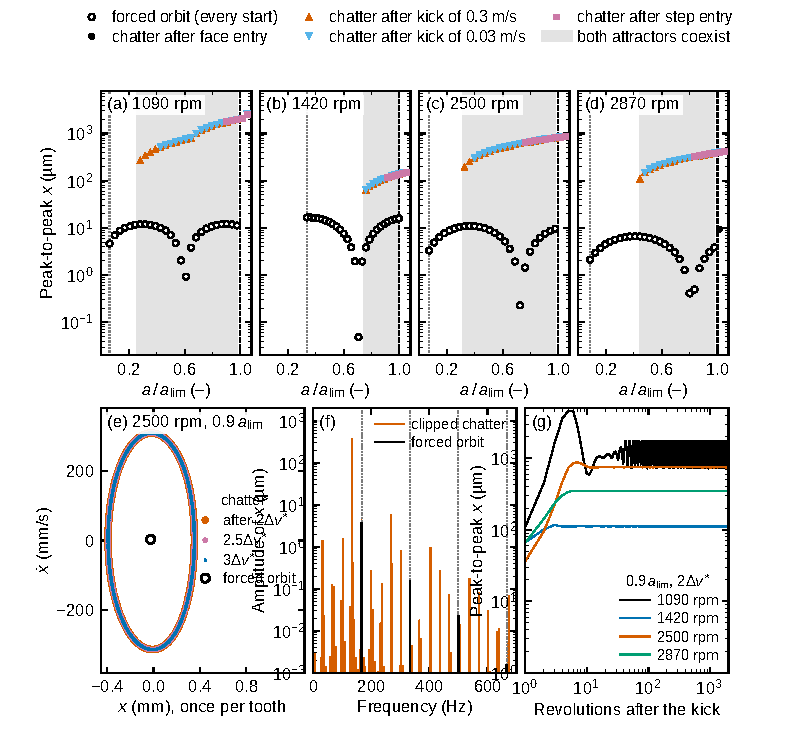
\includegraphics[width=\textwidth]{figures/fig_attractors.pdf}
  \caption{What lies beyond the basin ($g=\SI{1500}{\volt\second\per\metre}$, $\lvert V\rvert\le\SI{9}{\volt}$, full surface memory). (a)--(d)~Steady peak-to-peak displacement over the last 300 of 1600 revolutions against $a/\alim$, for four starts: open circles, the forced orbit, which every start reaches where it is the only attractor; filled markers, bounded chatter. Shaded: both attractors coexist; dotted: $\alim(0)$; dashed: $\alim$. (e)~Once-per-tooth samples of $(x,\dot x)$ of the last 500 tooth periods after kicks of 2, 2.5 and 3 times the critical kick, at \SI{2500}{\rpm} and $0.9\alim$: the three runs settle on the same closed curve around the forced orbit. (f)~Amplitude spectra of $x$ over 500 revolutions at the same point; dotted: tooth-passing harmonics. (g)~Peak-to-peak displacement per revolution after a kick of twice the critical kick at $0.9\alim$.}
  \label{fig:attr}
\end{figure}

\subsection{A describing-function prediction}\label{sec:bistab-df}

The size of the basin near the limit can be predicted with a dual-input describing function \citep{gelb1968describing}; actuator saturation in active vibration control of milling has also been modelled in the frequency domain by \citet{ozsoy2025frequency}, and whether that model already contains the forced command and a threshold amplitude, and so how far the estimate below goes beyond it, was not examined. Near the limit the deviation from the orbit is dominated by the chatter mode, and the unclipped command is $u=b(t)+A\sin\omega_ct$, with $A$ the amplitude of its chatter component and $\omega_c$ the chatter frequency. For $\omega_c$ incommensurate with $\omega_T$, the clip acts on the chatter component as the gain
\begin{equation}\label{eq:df}
  \mathcal N(A)=\lim_{\tau_a\to\infty}\frac{2}{A\tau_a}\int_0^{\tau_a}\operatorname{sat}_{V_{\max}}\bigl(b(t)+A\sin\omega_ct\bigr)\sin\omega_ct\,\mathrm dt\ \le 1,
\end{equation}
and the clipped loop thus behaves like DVF with the effective gain $\mathcal N(A)\,g$. A cut of depth $a<\alim(g)$ needs only the gain $g_e(a)$, the largest gain not above $g$ with $\alim(g_e)=a$, and chatter can be sustained once the gain of Eq.~\eqref{eq:df} falls below $g_e(a)/g$, i.e.\ above a critical amplitude $A^*(a)$. A kick $\Delta v$ excites the chatter mode with a velocity amplitude $p\,\Delta v$, where $p$ was fitted on the unclipped cut from the decay of its least-damped mode after a small kick (Supplementary Material). Hence
\begin{equation}\label{eq:dfbasin}
  \Delta v^*_{\mathrm{DF}}(a)=\frac{A^*(a)}{g\,p},\qquad
  \Delta v^*_{\mathrm{DF}}\;\to\;\frac{V_{\max}-b_{\max}}{g\,p}\quad\text{as }a\to a_{\lim},
\end{equation}
the limit holding because $g_e\to g$ and $\mathcal N(A)=1$ as long as $\bmax+A\le\Vmax$.
% src: src/c1_unsafe_zone.py (df_gain: 128 phases, b on 128 samples per tooth period; critical_amplitude; effective_gain_needed; _mode_factor: kick of 1 mm/s at phase 0, high-pass 40 Hz, fit of the slowest decaying mode)

Where $p$ could be fitted, from 0.7--$0.8\alim$ upwards, the simulated critical kick (median over the phases) is 0.61--1.13 times this estimate, and 0.88--1.13 times at 0.95 and $0.98\alim$ (Fig.~\ref{fig:basin}). Equation~\eqref{eq:dfbasin} predicts that the basin does not close at the limit but tends to a finite size, set by the voltage that the forced command leaves free; this is a prediction of the describing function, not a proven property of the basin at the limit itself. At $\alim$ the residual authority is $\Vmax-\bmax=3.9$, 1.7, 0.87 and \SI{4.7}{\volt} at 1090, 1420, 2500 and \SI{2870}{\rpm}, and at $0.999\alim$ the simulated critical kick is still 1.4--\SI{10.5}{\milli\metre\per\second} at the three speeds tested (Supplementary Material). The basin would close below $\alim$ only where $\bmax$ reached $\Vmax$; the authority condition of Section~\ref{sec:feasibility} keeps $\bmax\le\Vmax$ up to $\kappa\alim$, but with equality at some depth at the 94 speeds (1530--\SI{2460}{\rpm}) where the steady demand binds (Sections~\ref{sec:feas-res} and~\ref{sec:cert-c2}). This residual authority is fragile against persistent forcing that adds to $b$, such as runout (Section~\ref{sec:delayed-robust}). The estimate is cheap, but it rests on the filtering hypothesis and on the factor $p$, fitted at one kick phase and valid only near the limit; $A^*$ is the harmonic-balance amplitude of the unstable limit cycle that bounds the basin.
% src: results/c1_df.npz (A_dual at a = a_lim: 3.92, 1.66, 0.87, 4.69 V at 1090, 1420, 2500, 2870 rpm = V_max - b_max; the 1420 rpm value was 0.009 V before a round-off fix in c1_unsafe_zone.critical_amplitude, tests/test_c1_results.py), results/c1_basin.npz (p_mode finite at frac >= 0.7, at 1420 rpm >= 0.8), results/c1_summary.json (td_over_df 0.61-1.13); ratios at 0.95/0.98 recomputed with the c1_summary formula: 0.88-1.13; verification/tdsim/check11_kick_near_limit.json (1.405-1.467, 7.055-7.611, 9.150-10.533 mm/s); README §11.5; verification/paper/revision_runs.json (closed_form.runout_to_clip_g1500: 0.730, 3.09, 8.74 um at 2500, 2870, 1420 rpm; 1090 rpm below 9 V up to 10 um; worst command over 40 depths up to 0.9 a_lim and 8 runout phases, c4_robust.worst_orbit_command)

\begin{figure}[!tbp]
  \centering
  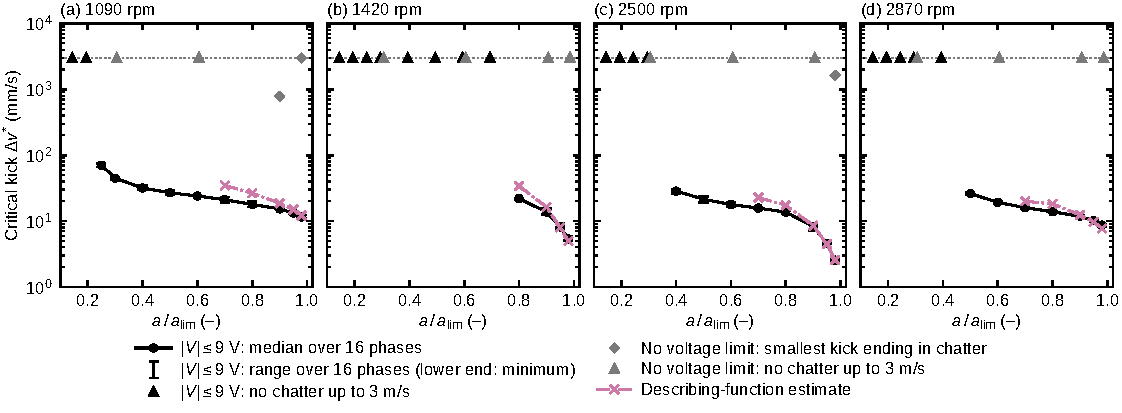
\includegraphics[width=\textwidth]{figures/fig05_basin.pdf}
  \caption{Critical kick $\Delta v^*$ against $a/a_{\lim}$ at (a)~1090, (b)~1420, (c)~2500 and (d)~\SI{2870}{\rpm} ($g=\SI{1500}{\volt\second\per\metre}$). With the \SI{9}{\volt} clip: median over 16 phases (circles) and range over the phases (bars; lower end: worst phase); black triangles: no chatter for any kick up to \SI{3}{\metre\per\second}. Without the clip: smallest kick that ends in chatter (diamonds) or no chatter up to \SI{3}{\metre\per\second} (grey triangles). Crosses: describing-function estimate, Eq.~\eqref{eq:dfbasin}. Right axis of (d): the kick as an equivalent displacement $\Delta v^*/\omega_n$.}
  \label{fig:basin}
\end{figure}

\subsection{Depth limit against the gain}\label{sec:bistab-gain}

At 1090 and \SI{2500}{\rpm} the entry limits were also computed for $g$ up to \SI{3000}{\volt\second\per\metre}. With the step entry the clipped limit nearly stops rising above about \SIrange{1500}{1650}{\volt\second\per\metre}, at about 19.8 and \SI{13.2}{\milli\metre}, while $\alim$ reaches 41.8 and \SI{40.0}{\milli\metre} at $g=3000$; the face entry follows $\alim$ until the forced command itself exceeds the clip (Supplementary Material). At large gains the depth at these two speeds is thus limited by the basin, which the entry transient exceeds, and not by the gain. Below the plateau the clipped step-entry limit rises with the gain, at \SI{2500}{\rpm} from \SI{6.4}{\milli\metre} at the reproduced gain of Eq.~\eqref{eq:pub} (\SI{536}{\volt\second\per\metre}), so in this model clipping a larger gain does not weaken DVF; the clipped-DVF comparison of \citet[Table~3]{ozsoy2026robust}, whose clipped gain is set by a tuning rule, was not reproduced.
% src: results/c1_gainplane.npz (a_step_clip, a_edge_clip, a_lim, orbit_peak_V), results/c1_summary.json (gainplane: step_clip_plateau_mm 19.78 and 13.19, a_lim_at_3000 41.82 and 40.03, orbit_saturates_from_g 3000 and 1650); README §11.6, §13.6; results/table3_main.csv (2500 rpm: a_prop_td 6.37 mm at the reproduced gain 535.6 V s/m; a_clip3000_td 13.23 mm), table3_clip_gain_sweep.csv; a_step_clip of c1_gainplane.npz rises monotonically with g at both speeds; README §5.5

\subsection{Checks of the protocols}\label{sec:bistab-checks}

\NEWCHECKS
